\documentclass[a4paper,10pt]{article}
\usepackage[utf8]{inputenc}
\usepackage[UKenglish]{babel}
\usepackage{fancyhdr}
\usepackage{anysize}
\usepackage{amsmath, amsthm, amssymb}
\usepackage{lastpage}
\usepackage[all]{xy}  % drawings
%\usepackage{listings} % code highlighting
\usepackage[usenames,dvipsnames]{color}
\usepackage{graphicx}
\usepackage{caption}
\usepackage{hyperref}

\pagestyle{fancy}
\fancyfoot[R]{\em \thepage / \pageref{LastPage}}
\fancyfoot[C]{}
\fancyfoot[L]{\em Master VIBOT}
\fancyhead[R]{\em Lab0 - Introduction to ROS}
\fancyhead[C]{}
\fancyhead[L]{\em Probabilistic Robotics}
\renewcommand{\headrulewidth}{0.4pt}
\renewcommand{\footrulewidth}{0.4pt}

%\,	 a small space
%\:	 a medium space
%\;	 a large space
%\quad	 a really large space
%\qquad	 a huge space
%\!	 a negative space (moves things back to the left)
        
\begin{document}

\marginsize{2cm}{2cm}{2cm}{2cm}

% Title
%\hspace{1mm}
\begin{center}
\Large \textbf{Lab0 - Introduction to ROS}
\end{center}
%\hspace{1mm}

\section{The goal}

The goal of this lab session is to get started with ROS that will be used used in all the lab sessions of Probabilistic Robotics. The Robot Operating System (ROS) is a software framework for robot software development. ROS provides libraries and tools to help software developers create robot applications. It provides hardware abstraction, device drivers, libraries, visualizers, message-passing, package management, and more. ROS will be used in the next lab exercises, so it is fundamental to understand all the basics given in this session. 

\section{Pre-lab: Installing Ubuntu and ROS}

Currently the only official supported platform for ROS is Ubuntu. Ubuntu is a computer OS (Operating System) based on Debian Linux. As the computers in the Robotics Lab doesn't have Ubuntu installed, the firsts steps you need to do is install Ubuntu and ROS in your machines. In order to install Ubuntu you can either:

\begin{enumerate}
    \item (prefered) Install Ubuntu in a partition alongside your other OS (hard disk install). Make sure that you install the distributions specified below:
    \begin{itemize}
        \item Ubuntu 12.04.5 LTS (\href{http://releases.ubuntu.com/12.04/ubuntu-12.04.5-desktop-amd64.iso}{download iso}).
        \item ROS Hydro Desktop Full install (\href{http://wiki.ros.org/hydro/Installation/Ubuntu}{install instructions}).
    \end{itemize}
    
    \item (not recommended) Install Ubuntu in a virtual machine inside your normal OS. In this case you can donwload a \href{https://www.virtualbox.org/wiki/Linux_Downloads}{Virtualbox}  and follow the same installation instruction than the previous point, but this time on the virtual machine. Note that this kind of installation can lead to problems with graphics drivers in some or all labs.
\end{enumerate}

\section{Lab: ROS tutorials}
Now that we have Ubuntu and ROS successfully installed, please follow the most fundamental ROS tutorials. Please have in mind that your ROS workspace, the place where you need to put all your packages is the catkin{\textunderscore}ws folder inside the home directory.

\begin{itemize}
    \item Creating a workspace for catkin.\\
    \url{http://wiki.ros.org/catkin/Tutorials/create_a_workspace}
    
    \item Navigating the ROS FileSystem.\\
    \url{http://wiki.ros.org/ROS/Tutorials/NavigatingTheFilesystem}
    
    \item Creating a ROS package.\\
    \url{http://wiki.ros.org/ROS/Tutorials/CreatingPackage}
    
    \item Understanding ROS Nodes.\\
    \url{http://wiki.ros.org/ROS/Tutorials/UnderstandingNodes}
    
    \item Understanding ROS topics.\\
    \url{http://wiki.ros.org/ROS/Tutorials/UnderstandingTopics}
    
    \item Understanding ROS services and Parameters.\\
    \url{http://wiki.ros.org/ROS/Tutorials/UnderstandingServicesParams}
    
    \item Writing a simple Publisher and subscriber (Pyhton).\\
    \url{http://wiki.ros.org/ROS/Tutorials/WritingPublisherSubscriber(python)}
    
    \item Examining the Simple Publisher and Subscriber.\\
    \url{http://wiki.ros.org/ROS/Tutorials/ExaminingPublisherSubscriber}
\end{itemize}
\noindent
Please note that the ROS Cheat Sheet, you can find in the files for this Lab might be useful for you.

\subsection{Turtlesim Waypoint Node}
During the Lab session you will need to create a node to interact with the turtle simulator seen in Understanding ROS nodes tutorial.
Run again turtlesim:
\begin{verbatim}
    roscore
\end{verbatim}
\noindent
In a new terminal:
\begin{verbatim}
    rosrun turtlesim turtlesim_node
\end{verbatim}

\begin{center}
    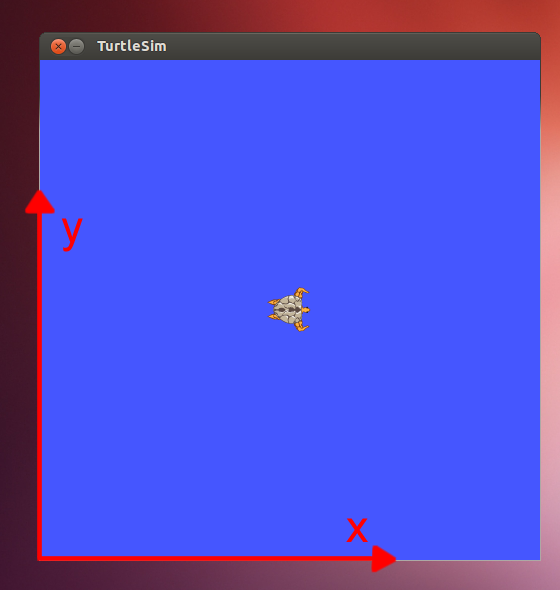
\includegraphics[width=0.2\textwidth]{pict/lab0}
    \captionof{figure}{Turtlesim visualization.}
    \label{sim}
\end{center}

\noindent
And using the ROS tools you’ve seen in the tutorials (rostopic, rosmsg, rqt{\textunderscore}graph) identify:
\begin{enumerate}
    \item The name of the topic used to send velocity commands to the turtle and the type of these messages.
    \item The name of the topic where the turtle position it is published at, and the type of these messages.
\end{enumerate}

\noindent
Clone the repository of the Probabilistic labs in your workspace. This repository contains all the code for this labs. After download compile the code:
\begin{verbatim}
    cd ~/catkin_ws/src
    git clone https://bitbucket.org/gvallicrosa/probabilistic_labs.git
    cd ~/catkin_ws
    catkin_make
\end{verbatim}
\noindent Remember before starting any lab to update the repos with:
\begin{verbatim}
    cd ~/catkin_ws/src/probabilistic_labs
    git pull
    cd ~/catkin_ws
    catkin_make
\end{verbatim}
\noindent
Run the node in the turtle{\textunderscore}waypoint package: 
\begin{verbatim}
    rosrun lab0_ros turtle_waypoint.py
\end{verbatim}
You will see that nothing happens. You need to modify the \emph{turtle{\textunderscore}waypoint.py} node inside the package in order to publish commands to the turtle to make it go to a desired point. This desired position will be specified when running the node through the command line like:
\begin{verbatim}
 	 rosrun lab0_ros turtle_waypoint.py 1.2 5.0
\end{verbatim}
being the desired point is x: 1.2, y: 5.0. If the point is not given when calling the node, the node will check the ROS parameter server for the parameters \emph{/default{\textunderscore}x} and \emph{/default{\textunderscore}y} and head to that point. In the case that the parameters are not set the turtle won't move. You can set ROS parameters like:
\begin{verbatim}
    rosparam set default_x 5
    rosparam set default_y 10
\end{verbatim}

\section{Lab report}

After the lab session: Write a brief report (max 2 pages) explaining your solution and problems faced. Include the final \emph{turtle{\textunderscore}waypoint.py} file.

\end{document}
